%!TEX TS-program = xelatex
\documentclass[]{friggeri-cv}
\usepackage{afterpage}
\usepackage{hyperref}
\usepackage{color}
\usepackage{xcolor}
\hypersetup{
	pdftitle={},
	pdfauthor={},
	pdfsubject={},
	pdfkeywords={},
	colorlinks=false,       % no lik border color
	allbordercolors=white    % white border color for all
}
\addbibresource{bibliography.bib}
\RequirePackage{xcolor}
\definecolor{pblue}{HTML}{0395DE}

\begin{document}
	\header{Rohit}{Kumar}
	{Researcher}
	
	% Fake text to add separator      
	\fcolorbox{white}{gray}{\parbox{\dimexpr\textwidth-2\fboxsep-2\fboxrule}{%
			.....
	}}
	
	% In the aside, each new line forces a line break
	\begin{aside}
	  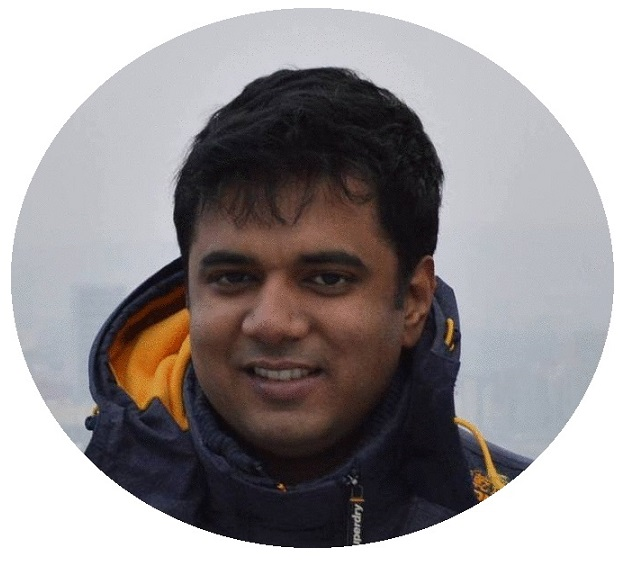
\includegraphics[scale=0.30]{img/meg2.jpg}
		~
		\section{Mail}
		\href{mailto:rohit.kumar@eurecat.org}{rohit.kumar@eurecat.org}
	\href{mailto:rohit1308k@gmail.com}{rohit1308k@gmail.com}
		~
		\section{Web \& Git}
		\href{https://www.linkedin.com/in/rohit13k/}{linkedin.com/in/rohit13k/}
	\href{rohit13k.github.io}{rohit13k.github.io}
	\href{https://github.com/rohit-nlp}{https://github.com/rohit-nlp}
		~
		\section{Programming}
			\textbf{Java}
\includegraphics[scale=0.40]{img/5stars.png}
		\textbf{Scala}
\includegraphics[scale=0.40]{img/4stars.png}
		\textbf{Python}
\includegraphics[scale=0.40]{img/3stars.png}
		~
		\section{Big Data Systems}
		\textbf{Spark}
\includegraphics[scale=0.40]{img/5stars.png}
		\textbf{Hadoop}
\includegraphics[scale=0.40]{img/4stars.png}
		\textbf{Kafka}
\includegraphics[scale=0.40]{img/3stars.png}
		\textbf{NoSQL}
\includegraphics[scale=0.40]{img/3stars.png}
		~
		\section{Personal Skills}
		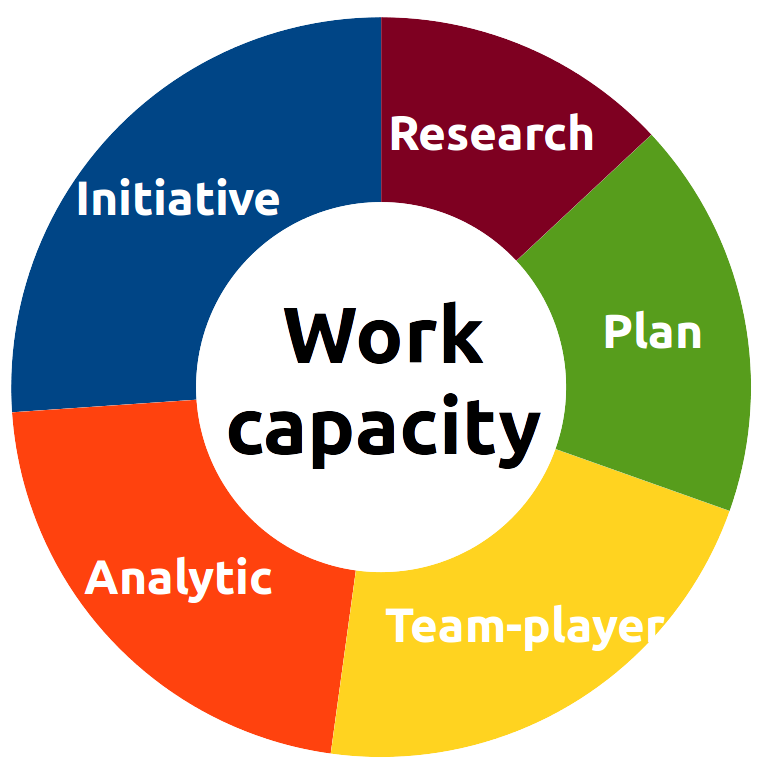
\includegraphics[scale=0.62]{img/personal.png}
		~
	\end{aside}
	
	\section{Experience}
	\begin{entrylist}
	 \entry
	{07/18 - Now}
	{Researcher}
	{Eurecat, Barcelona, Spain}
	{Working as Researcher and Big Data Architect in the Big Data analytics group in Eurecat. Working in multiple projects providing consulting and development support for big data tools such as: \\
	- Big Data Architect: Designed the big data platform for a supermarket chain in Spain to help them migrate from their traditional in house data ware system to an on cloud data lake for big data analytical
	use cases.
	\\- Big Data Architect: Designed and helped in the development of a new platform for an advertising company in Madrid for storing user web clickstream data and providing recommendation and predictions using Spark.
	\\- Big Data Engineer: Developed a plugin in ElasticSearch for data clustering to be used in an EU search platform.
	\\- Big Data Engineer: Developed and helped redesign the Data visualization platform BCNNow as part
	of DECODE project.
	\\- Researcher: Working on Data privacy tool for an EU Project SMOOTH to help Micro and Small
	enterprises with GDPR compliance.
	\\- Research Engineer: Worked on developing a large social graph mining engine Kalium using OrientDB
	and Spark.
	\\- Big Data Engineer: Maintain and support the inhouse cloud for Eurecat using Red Hat Openstack
	Platform.}
	\entry
	{08/14 - 06/18}
	{Big Data Enginner}
	{Upwork (Freelance)}
	{ Worked on multiple short and long term projects for multiple clients on big data and data science domain.\\
		- Spark NLP: Core developer to develop and support the Spark NLP library.\\
		- Disperse.io: Worked on analyzing and discovering trends in Wi-Fi data for London metro stations. Worked as data engineer in data cleaning and data analysis using Spark-SQL.\\
		- Discovergy: Worked on smart meter applications. Developed a machine learning based platform on top of Spark streaming to collect, store and analysis data from smart meters. \\
		- L3Networks: Designed and implemented a processing system that could process web logs arriving at the rate of 46GB/min in real-time. Designed the architecture and the data processing pipeline using Apache Kafka, Apache Spark and Apache Hadoop using Java and Scala Languages. The work included deployment of these technologies as well.\\
		- DigitalVidya: Designed and delivered online course on Big Data Engineering course (Hadoop, Spark, Hive, Pig, Cassandra, NoSQL) for DigitalVidya for 3 batches of 10 students. Delivered two course on Data Science with Python (NumPy, Pandas, scikit-learn) and R.\\
	}		
\end{entrylist}
	\begin{entrylist}
	\entry
	{06/14 - 07/14}
	{Software Designer}
	{Royal bank of Scotland, Delhi, India}
	{Developed data pipelines for the massive amount of banking and trading data for RBS using in-memory database on Oracle Coherence. \\}

	\entry
	{04/11 - 05/14}
	{Assistant Consultant}
	{Tata Consultancy Services, Mumbai, India}
	{Technical team lead and Scrum Master for the entire online assessment platform, an online cloud based system for conducting online examinations and certifications. As technical lead I was responsible for 10 different products on the assessment platform and was supervising a team of 30 developers.\\
		I was the lead architect and developer for the deployment of the complete eco-system of the online assessment platform in multi-tenant architecture for software as a service model. I also contributed as technical expert in pre sales and helped in designing new product offerings for the education domain. \\
		Technologies used: J2EE, Java, MySQL, SVN, Struts 2, Hibernate, Memcached, Adobe Flex\\
	}
	\entry
	{03/11 - 09/11}
	{Researcher}
	{Tata Research Development and Design Center, Pune, India}
	{Worked on data privacy and data security. Worked on data masking techniques for privacy preserving data mining. \\
		Technologies used: C++, CVS\\}
	\end{entrylist}
	
	\section{Education}
	\begin{entrylist}
		 \entry
		{2014 - 2018}
		{Ph.D Candidate}
		{Universit\'{e} Libre de Bruxelles \&  Universitat Polit\'{e}cnica de Catalunya}
		{Done a joint PhD from ULB and UPC under joint supervision from Toon Calders and Alberto Abello, Funded by FNRS scholarship.\\}
		
		\entry
		{2008 - 2011}
		{M.Sc in Computer Science}
		{Chennai Mathematical Institute, India}
		{The Master course was done part time while working in TCS.
			Main subjects: Discreet Mathematics, Database Systems, Operating systems, Data mining, Cryptography, Statistics, Design and Analysis of Algorithm,
			Theory of Computation, Programming language Concepts. Grade: \textbf{8.44\%}\\
			Thesis: Security aspects of online Assessment platform-Touchstone.\\}
		\entry
		{2004 - 2007}
		{B.Sc (Hons) in Physics}
		{Hindu College, Delhi University}
		{Did summer research internship at IISC Bangalore every summer break. Co-Organized Physics Department fest on 2006.
			Percentage: \textbf{76.1\%}\\}
	\end{entrylist}
	
	\section{Awards and Achievements}
	\begin{entrylist}
		\entry
		{2019}
		{Big Data Talent Awards}
		{BigDataCoE}
		{Awarded Best PhD in Big Data in Catalonia, Spain for year 2018.}
		 \entry
		{2013}
		{Best Technical Lead Award in ACTion2013 in SMB iON}
		{TCS}
		{Awarded best technical lead in the entire department of 500 developers and 25 teams.\\}
		\entry
		{2011}
		{Innovation of the year award southern region}
		{Tata Innovista}
		{Tata group yearly award for innovations across the Tata groups  companies.\\}
	\end{entrylist}
	
	


	
	%%% This piece of code has been commented by Karol Kozioł due to biblatex errors. 
	% 
	%\printbibsection{article}{article in peer-reviewed journal}
	%\begin{refsection}
	%  \nocite{*}
	%  \printbibliography[sorting=chronological, type=inproceedings, title={international peer-reviewed conferences/proceedings}, notkeyword={france}, heading=subbibliography]
	%\end{refsection}
	%\begin{refsection}
	%  \nocite{*}
	%  \printbibliography[sorting=chronological, type=inproceedings, title={local peer-reviewed conferences/proceedings}, keyword={france}, heading=subbibliography]
	%\end{refsection}
	%\printbibsection{misc}{other publications}
	%\printbibsection{report}{research reports}
	
\end{document}
